\section{Experiments}%

\label{sec:experiments}

We evaluate the performance of \method in part segmentation and articulation estimation for both rest and articulated states.
Our experiments mainly answer three questions:
(1) whether two-state reasoning improves the model generalization over single-state reasoning;
(2) whether the network achieves consistent predictions between two states and whether the Siamese framework further improves the consistency;
and (3) whether the recovered articulation is good enough to be exported as a URDF asset for downstream robot simulation.
We first describe the evaluation protocol, then report comparisons with state-of-the-art methods, ablations, and an application in RoboTwin.

\begin{table}[t]
\centering
\small
\caption{
\textbf{Evaluation on rest and fully articulated states.}
For each dataset we report rest-pose segmentation (gIoU, part-wise Chamfer distance PC, and mIoU) and articulated geometry (gIoU, PC, and whole-object Chamfer distance OC).
All metrics are computed with penalties applied to unmatched parts.
--: method is not applicable for the articulated state.
1@10: best sample out of 10 predictions per instance.
Colors: \best{best} and \secondbest{second best}.
}%
\label{tab:combined-comparison}
\setlength{\tabcolsep}{3pt}
\renewcommand{\arraystretch}{1.1}
\resizebox{\linewidth}{!}{%
\begin{tabular}{@{}lcccccc ccccccc@{}}
\toprule
& \multicolumn{6}{c}{\textbf{Lightwheel}}
& \multicolumn{6}{c}{\textbf{PartNet-Mobility}} \\
\cmidrule(lr){2-7}\cmidrule(lr){8-13}
\textbf{Method} & \multicolumn{3}{c}{\textbf{Rest-Pose Seg.}}
& \multicolumn{3}{c}{\textbf{Articulated States}}
& \multicolumn{3}{c}{\textbf{Rest-Pose Seg.}}
& \multicolumn{3}{c}{\textbf{Articulated States}} \\
\cmidrule(lr){2-4}\cmidrule(lr){5-7}\cmidrule(lr){8-10}\cmidrule(lr){11-13}
& gIoU$\uparrow$ & PC$\downarrow$ & mIoU$\uparrow$
& gIoU$\uparrow$ & PC$\downarrow$ & OC$\downarrow$
& gIoU$\uparrow$ & PC$\downarrow$ & mIoU$\uparrow$
& gIoU$\uparrow$ & PC$\downarrow$ & OC$\downarrow$ \\
\midrule
% PartField~\cite{liu2025partfield}
%   & 0.079 & \best{0.106} & 0.264
%   & -- & -- & --
%   & 0.183 & 0.123 & 0.361
%   & -- & -- & -- \\
P3SAM~\cite{ma2025p3sam}
  & 0.122 & 0.177 & 0.411
  & -- & -- & --
  & -0.116 & 0.261 & 0.267
  & -- & -- & -- \\
\midrule
SINGAPO~\cite{liusingapo}
  & -0.097 & 0.234 & 0.273
  & -0.102 & 0.329 & 0.018
  & 0.262 & 0.124 & 0.468
  & 0.255 & 0.184 & 0.046 \\
SINGAPO~\cite{liusingapo} (1@10)
  & -0.050 & 0.221 & 0.297
  & -0.056 & 0.261 & 0.019
  & 0.271 & 0.117 & 0.471
  & 0.264 & 0.168 & 0.041 \\
Articulate AnyMesh~\cite{qiu2025articulate}
  & 0.172 & 0.190 & 0.452
  & 0.158 & 0.237 & 0.010
  & 0.383 & 0.104 & 0.542
  & 0.378 & 0.251 & 0.022 \\
Particulate~\cite{li2025particulate}
  & 0.332 & \secondbest{0.168} & 0.576
  & 0.305 & 0.208 & 0.009
  & {0.880} & \secondbest{0.003} & {0.884}
  & {0.843} &{0.022} & \secondbest{0.003} \\
\textbf{\method (Single)}
  & \secondbest{0.489} & \best{0.156} & \secondbest{0.578}
  & \secondbest{0.474} & \secondbest{0.194} & \best{0.003}
  & \secondbest{0.924} & \best{0.002} & \secondbest{0.936}
  & \secondbest{0.888} &\secondbest{0.007} & \best{0.001} \\
\textbf{\method (Siamese)}
  & \best{0.544} & \best{0.156} & \best{0.647}
  & \best{0.512} & \best{0.188} & \secondbest{0.005}
  & \best{0.931} & \secondbest{0.003} & \best{0.939}
  & \best{0.890} & \best{0.005} & \best{0.001} \\
\bottomrule
\end{tabular}%
}
\end{table}


\subsection{Experimental Setup}
\label{sec:exp_setup}

\heading{Training Datasets}
We train \method on the PartNet-Mobility~\cite{Mo_2019_CVPR} and GRScenes~\cite{wang2024grutopia} datasets.
For PartNet-Mobility, we follow the train-test split of SINGAPO~\cite{liusingapo}; for GRScenes, we use all articulated assets for training.
We set the maximum number of parts to $K_{\max}=16$ and discard objects with more than 16 articulated parts, yielding 3,800 training objects across 50 categories.

\heading{Testing Datasets}
For evaluation, we use the PartNet-Mobility test split, which contains 7 common articulated-object categories, and the Lightwheel benchmark~\cite{lightwheel_simready_2025}, which contains 243 high-quality articulated objects spanning 14 categories.
For every object, we sample two distinct physical states and convert them into a pair of unorganized point clouds.
Since the two point clouds are sampled independently, the model does not rely on explicit point correspondence between the states.


% \heading{Baselines.}
% We compare against representative methods for segmentation, retrieval-based reconstruction, and feed-forward articulation inference.
% The baselines include a naive part-matching baseline, SINGAPO~\cite{liusingapo}, PartField~\cite{liu2025partfield}, P3SAM~\cite{ma2025p3sam}, Articulate AnyMesh~\cite{qiu2025articulate}, and Particulate~\cite{li2025particulate}.
% For methods that can benefit from mesh connectivity, we report connectivity-assisted variants marked by $^\dagger$.
% This protocol separates the effect of geometric connectivity from the ability to infer articulation from the observed states.

\heading{Implementation details}
Each input state is represented by a point cloud sampled from the corresponding mesh.
Following Particulate~\cite{li2025particulate}, we augment point coordinates with surface normals and PartField features.
At test time, \method uses a single forward branch to predict the part masks, kinematic tree, motion type, joint axes, and motion ranges, \ie, the reverse-order branch and cycle-consistency objective are used only during training. Training the main model takes approximately three days on 4 NVIDIA H100 GPUs. More details can be found in~\Cref{sec:supp_data_processing}.

\heading{Metrics}
We evaluate both part recovery and articulated reconstruction quality.
For evaluation on the rest state, we report generalized IoU (gIoU), part-wise Chamfer distance (PC), and mean IoU (mIoU) between predicted and ground-truth parts.
For evaluation on the articulated state, we actuate the predicted parts using the predicted joint parameters and report part-wise gIoU, PC, and the whole-object Chamfer distance (OC).
The metrics in the articulated state are usually lower than in the rest state because errors in segmentation, kinematic hierarchy, joint axes, and motion range accumulate after actuation.
Unless otherwise stated, we use the penalty protocol for unmatched/missing parts as in~\cite {li2025particulate}, which discourages methods from producing visually plausible but incomplete decompositions.

\subsection{Main Results}
\label{sec:exp_results}

\heading{Part segmentation at the rest state}
\Cref{tab:combined-comparison} (\textbf{Res-Pose Seg.}) shows the quality of part decomposition in the rest state.
On both PartNet-Mobility and Lightwheel, \method achieves the best gIoU (0.544 \vs 0.322), PC (0.156 \vs 0.168), and mIoU (0.647 \vs 0.576) among the compared methods,
indicating that the second-observed state helps the network identify which geometry should move as a rigid part.
This improvement is especially important for articulated objects whose static geometry is ambiguous, such as cabinets with visually similar panels or appliances whose movable components are flush with the body.
% \cxz{refer to image example.}
As shown in~\Cref{fig:qualitative_results}, compared with single-state feed-forward baselines, the two-state formulation provides direct evidence of rigid part segmentation from relative motion rather than forcing the model to infer articulation only from category-level priors as in~\cite{li2025particulate}.

\begin{figure}[t]
  \centering
  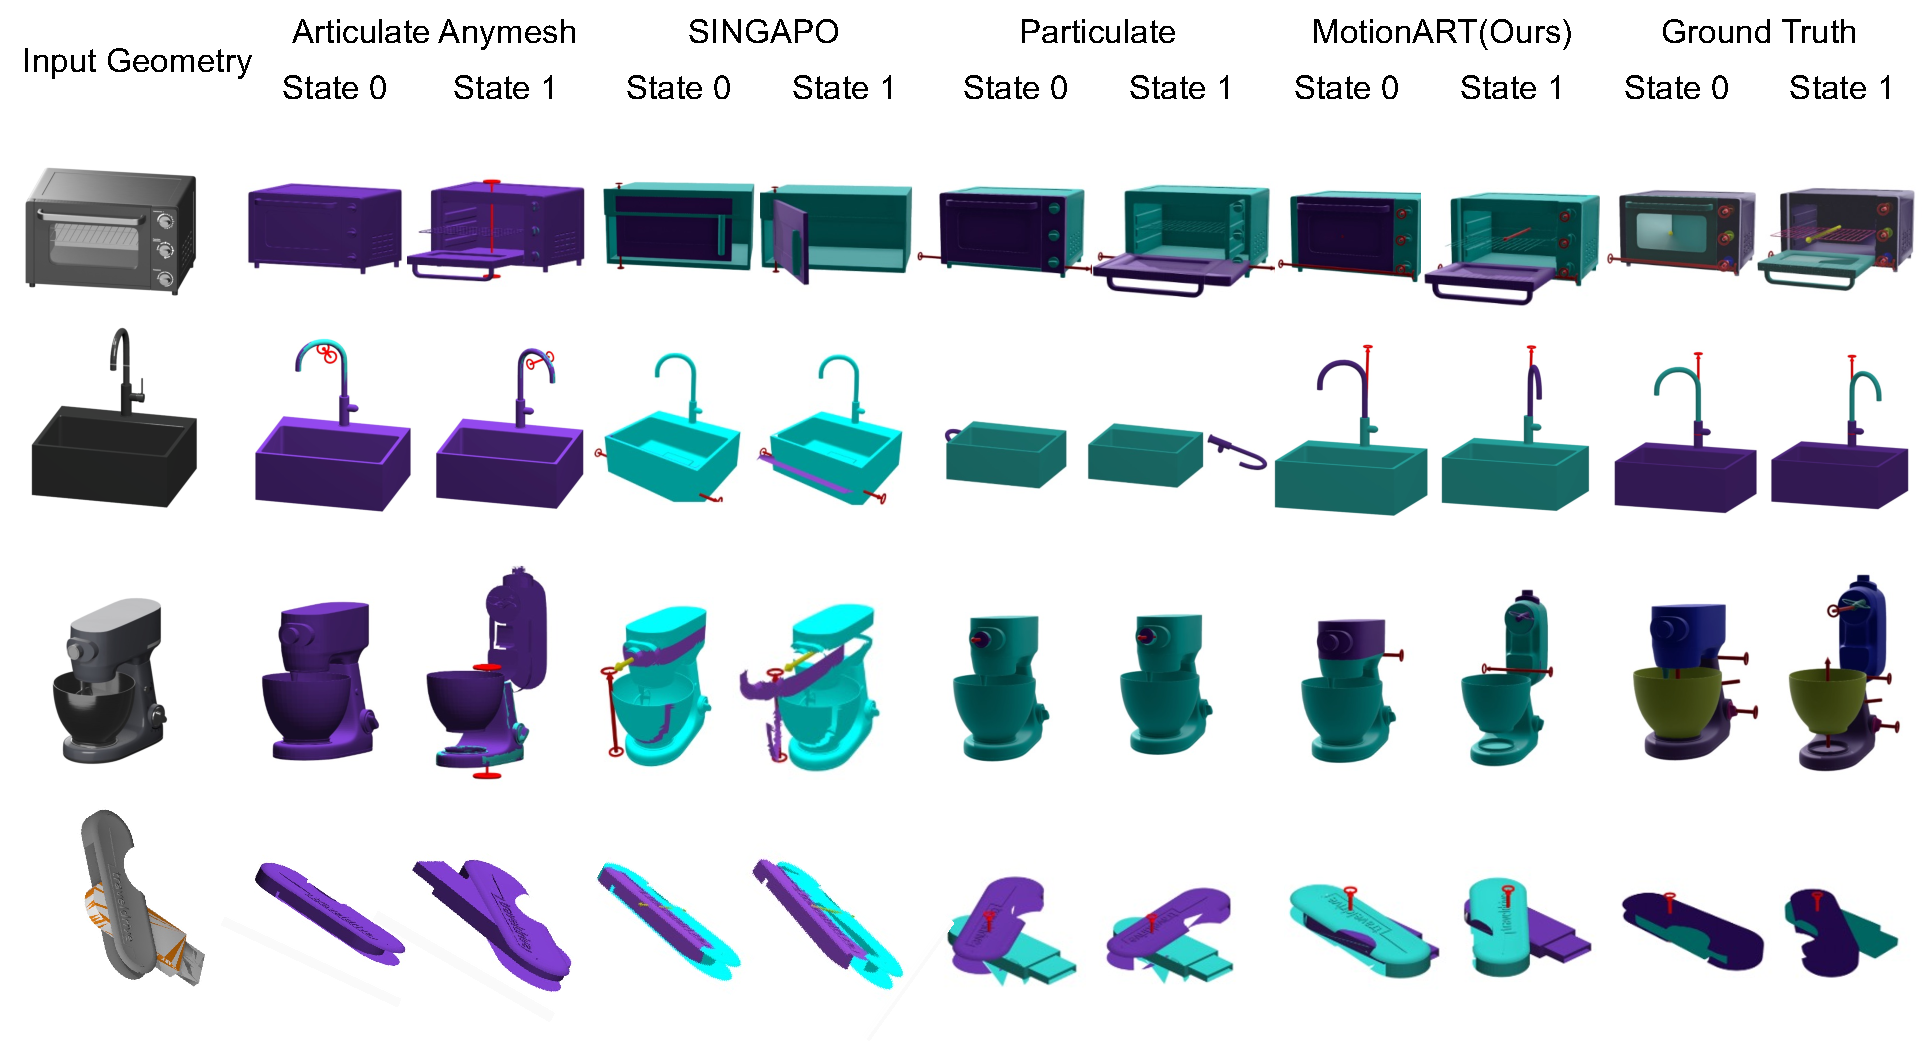
\includegraphics[width=\textwidth]{figs/results_compare.pdf}
  \caption{Qualitative comparison of articulation prediction. We visualize the articulated object in both the rest and fully articulated states. Given the same object, \method predicts more precise part segmentation and better articulation motion on both states than the state-of-the-art methods.}
  \label{fig:qualitative_results}
\end{figure}

% \begin{table}[t]
\centering
\small
\caption{
\textbf{Evaluation on the rest and fully articulated states.}
% For the fully articulated states, every part is moved to its maximum extent. 
We report generalized IoU (gIoU) and part-wise Chamfer distance (PC) for both states. Additionally, we report mean IoU (mIoU) for the rest of the states (computed with penalties for unmatched parts) and whole-object Chamfer distance (OC) for the fully articulated states (measuring the overall bidirectional Chamfer distance between the \emph{whole} predicted geometry and its GT counterpart).
--: SINGAPO assumes mesh connectivity between parts and is not applicable to the PartNet-Mobility test set.
1@10: computed using the best sample out of 10 predictions per instance.
Colors: \best{best} and \secondbest{second best}.
}%
\label{tab:combined-comparison}
% \vspace{-1em}
\setlength{\tabcolsep}{3pt}
\renewcommand{\arraystretch}{1.05}
% 引入 array 宏包并在导言区定义等宽的居中列，例如:
% \usepackage{array}
% \newcolumntype{C}{>{\centering\arraybackslash}p{1.9cm}}
% \resizebox{\linewidth}{!}{%
\begin{tabular}{@{}l *{6}{>{\centering\arraybackslash}p{1cm}} @{}}
\toprule
 & \multicolumn{3}{c}{\textbf{Lightwheel}} & \multicolumn{3}{c}{\textbf{PartNet-Mobility}} \\
\cmidrule(lr){2-4}\cmidrule(lr){5-7}
\textbf{Method}
& gIoU$\uparrow$
& PC$\downarrow$
& $\Delta$
& gIoU$\uparrow$
& PC$\downarrow$
& $\Delta$ \\
\midrule
\multicolumn{7}{c}{\textbf{(a) Rest States ($\Delta$: mIoU$\uparrow$)}} \\
\midrule
PartField~\cite{liu2025partfield} & 0.079 & \best{0.106} & 0.264  & 0.183 & 0.123 & 0.361 \\
P3SAM~\cite{ma2025p3sam}    & 0.122 & 0.177 & 0.411 & -0.116 & 0.261 & 0.267 \\
SINGAPO~\cite{liusingapo}   & -0.097 & 0.234 & 0.273 & 0.262 & 0.124 & 0.468 \\
SINGAPO~\cite{liusingapo} (1@10)  & -0.050 & 0.221 & 0.297 &   0.271 & 0.117 & 0.471 \\
Articulate AnyMesh~\cite{qiu2025articulate}   & 0.172 & 0.190 & 0.452 & 0.383 & 0.104 & 0.542 \\
Particulate~\cite{li2025particulate} & \secondbest{0.332} & {0.168} & \secondbest{0.576} & \secondbest{0.880} & \secondbest{0.003} & \secondbest{0.884}\\
ours          & \best{0.544} & \secondbest{0.156} & \best{0.647} & \best{0.924} & \best{0.002} & \best{0.936} \\
\midrule
\multicolumn{7}{c}{\textbf{(b) Fully Articulated States ($\Delta$: OC$\downarrow$)}} \\
\midrule
SINGAPO~\cite{liusingapo}    & -0.102 & 0.329 & 0.018 &  0.255 & 0.184 & 0.046 \\
SINGAPO~\cite{liusingapo} (1@10)    & -0.056 & 0.261 & 0.019 &  0.264 & 0.168 & 0.041 \\
Articulate AnyMesh~\cite{qiu2025articulate}   & 0.158 & 0.237 & 0.010 & 0.378 & 0.251 & 0.022 \\
Particulate~\cite{li2025particulate}    & \secondbest{0.305} & \secondbest{0.208} & \secondbest{0.009} & \secondbest{0.843} & \secondbest{0.022} & \secondbest{0.003} \\
ours            & \best{0.512} & \best{0.188} & \best{0.005} & \best{0.888} & \best{0.007} & \best{0.001}\\
\bottomrule
\end{tabular}%
% } %
\end{table}
% 
\begin{table}[t]
\centering
\small
\caption{
\textbf{Evaluation on the rest states.}
We report generalized IoU (gIoU), part-wise Chamfer distance (PC), and mean IoU (mIoU), all computed with penalties applied to unmatched parts.
% $^\dagger$: leveraging mesh connectivity.
--: SINGAPO assumes mesh connectivity between parts and is not applicable to the PartNet-Mobility test set.
1@10: computed using the best sample out of 10 predictions per instance.
Colors: \best{best} and \secondbest{second best}.
}%
\label{tab:rest-comparison}
\vspace{-1em}
\setlength{\tabcolsep}{3pt}
\renewcommand{\arraystretch}{1.05}
% \resizebox{\linewidth}{!}{%
\begin{tabular}{@{}lcccccc@{}}
\toprule
 & \multicolumn{3}{c}{\textbf{Lightwheel}} & \multicolumn{3}{c}{\textbf{PartNet-Mobility}} \\
\cmidrule(lr){2-4}\cmidrule(lr){5-7}
%
\textbf{Method}
& gIoU$\uparrow$
& PC$\downarrow$
& mIoU$\uparrow$
& gIoU$\uparrow$
& PC$\downarrow$
& mIoU$\uparrow$ \\
%
% \midrule
%
% Naive Baseline & 0.018 & 0.285 & 0.413 & 0.296 & 0.210 & 0.612 \\
% SINGAPO~\cite{liusingapo}        & -0.116 & 0.201 & 0.272 & -- & -- & -- \\
% SINGAPO~\cite{liusingapo} (1@10)        & -0.096 & 0.190 & 0.277 & -- & -- & -- \\

\midrule
PartField~\cite{liu2025partfield} & 0.079 & \best{0.106} & 0.264  & 0.183 & 0.123 & 0.361 \\
P3SAM~\cite{ma2025p3sam}    & 0.122 & 0.177 & 0.411 & -0.116 & 0.261 & 0.267 \\
SINGAPO~\cite{liusingapo}   & -0.097 & 0.234 & 0.273 & 0.262 & 0.124 & 0.468 \\
SINGAPO~\cite{liusingapo} (1@10)  & -0.050 & 0.221 & 0.297 &   0.271 & 0.117 & 0.471 \\
Articulate AnyMesh~\cite{qiu2025articulate}   & 0.172 & 0.190 & 0.452 & 0.383 & 0.104 & 0.542 \\
Particulate~\cite{li2025particulate} & \best{0.332} & \secondbest{0.168} & \best{0.576} & \secondbest{0.880} & \secondbest{0.003} & \secondbest{0.884}\\


ours (single query)          & {0.489} & {0.163} & {0.578} & \best{0.924} & \best{0.002} & \best{0.936} \\
\bottomrule
\end{tabular}%
% } %
\end{table}



\heading{Articulated-state reconstruction}
\Cref{tab:combined-comparison} (\textbf{Articulated State}) evaluates whether the recovered articulation remains correct after applying the predicted motion.
\method achieves the best performance across all articulated-state metrics, including whole-object Chamfer distance (reducing it from 0.09 to 0.03, a 66\% improvement).
Because this evaluation actuates each predicted joint to its maximum extent, the result validates more than static segmentation: the predicted kinematic structure, motion type, axis, and range must be mutually consistent.
The gap between rest-state and articulated-state performance also reveals why the evaluation should include motion-based metrics; a method can segment parts reasonably while still producing an incorrect joint that fails after actuation.
\Cref{fig:qualitative_results} visualizes representative predictions across object categories.
All state-of-the-art methods struggle with the ``switch'' on ``microwave'',
the ``arm'' of the ``Mixer''.
\method better captures the motion of these small, protruding parts, which are often visually ambiguous in the rest state but become more distinguishable when observing how they move.
This supports the quantitative trend: observing how geometry changes gives the model a more reliable cue for separating functional parts and predicting their motion.

% 
\begin{table}[t]
\centering
\small
\caption{
\textbf{Evaluation on the fully articulated states}, where every part is moved to its maximum extent.
We report part-wise gIoU and PC as in \Cref{tab:rest-comparison}, and whole-object Chamfer distance (OC), which measures the overall bidirectional Chamfer distance between the \emph{whole} predicted geometry and its GT counterpart.
Notations --, 1@10: same as \Cref{tab:rest-comparison}.
Colors: \best{best} and \secondbest{second best}.
}
\vspace{-1em}
\label{tab:full-comparison}
\setlength{\tabcolsep}{3pt}
\renewcommand{\arraystretch}{1.05}
% \resizebox{\linewidth}{!}{%
\begin{tabular}{@{}lcccccc@{}}
\toprule
 & \multicolumn{3}{c}{\textbf{Lightwheel}} & \multicolumn{3}{c}{\textbf{PartNet-Mobility}} \\
\cmidrule(lr){2-4}\cmidrule(lr){5-7}
%
\textbf{Method} & gIoU$\uparrow$ & PC$\downarrow$ & OC$\downarrow$
& gIoU$\uparrow$ & PC$\downarrow$ & OC$\downarrow$ \\

% \midrule
% Naive Baseline & 0.016 & 0.293 & 0.017 & 0.296 & 0.216 & 0.027 \\
% SINGAPO~\cite{liusingapo}     & -0.121 & 0.299 & 0.011 & -- & -- & -- \\
% SINGAPO~\cite{liusingapo} (1@10)  & -0.100 & 0.238 & 0.012 & -- & -- & -- \\

\midrule
SINGAPO~\cite{liusingapo}    & -0.102 & 0.329 & 0.018 &  0.255 & 0.184 & 0.046 \\
SINGAPO~\cite{liusingapo} (1@10)    & -0.056 & 0.261 & 0.019 &  0.264 & 0.168 & 0.041 \\
Articulate AnyMesh~\cite{qiu2025articulate}   & 0.158 & 0.237 & 0.010 & 0.378 & 0.251 & 0.022 \\
Particulate~\cite{li2025particulate}    & \best{0.305} & \best{0.208} & \secondbest{0.009} & \secondbest{0.843} & \secondbest{0.022} & \secondbest{0.003} \\
ours (single query)           & {0.474} & {0.194} & \best{0.003} & \best{0.888} & \best{0.007} & \best{0.001}\\
\bottomrule
\end{tabular}%
% }
\end{table}

\begin{table}[tb!]
    \centering
    \caption{\textbf{Ablation study on model design choices.}
    % We evaluate the contribution of different input-state configurations and training objectives. 
    % In the single-branch setting, we compare models using different numbers of observed states and further ablate the attention mask. 
    % In the Siamese setting, we study the effect of the cycle-consistency loss and compare it with the final model. 
    The ablation is done using a subset of training and evaluation data.
    We report reconstruction quality on both the rest and articulated states, together with inference time. 
    Best results are highlighted in \textbf{bold}.}
    \label{tab:ablation}
    \renewcommand{\arraystretch}{1.0}

    \begin{tabular}{@{} l ccc ccc c @{}}
        \toprule
        \multirow{2}{*}{\textbf{Method}} 
        & \multicolumn{3}{c}{\textbf{Rest state}} 
        & \multicolumn{3}{c}{\textbf{Articulated state}} 
        & \multirow{2}{*}{\textbf{Time}} \\
        \cmidrule(lr){2-4} \cmidrule(lr){5-7}
        & gIoU$\uparrow$ & PC$\downarrow$ & mIoU$\uparrow$ 
        & gIoU$\uparrow$ & PC$\downarrow$ & OC$\downarrow$ 
        & \\
        \midrule

        \multicolumn{8}{l}{\underline{\textbf{Single branch}}} \\
        \textbf{1-state}     
        & {0.305} & {0.096} & {0.480} & {0.293} & {0.144} & {0.008} & {7s} \\
        
        \textbf{2-state (default)}    
        & {0.396} & {0.083} & {0.531} & {0.382} & {0.127} & \textbf{0.004} & {10s} \\
        
        \textbf{4-state}     
        & {0.440} & {0.074} & {0.565} & {0.424} & {0.092} & \textbf{0.004} & {15s} \\
        
        \textbf{8-state}     
        & {0.456} & \textbf{0.073} & {0.574} & \textbf{0.447} & \textbf{0.088} & \textbf{0.004} & {18s} \\
        
        \textbf{w/o attn. mask}  
        & {0.386} & {0.093} & {0.540} & {0.371} & {0.134} & {0.007} & {10s} \\ 

        \midrule 
        \multicolumn{8}{l}{\underline{\textbf{Siamese}}} \\
        
        \textbf{w/o cycle loss} 
        & {0.419} & {0.085} & {0.560} & {0.403} & {0.127} & {0.005} & {10s} \\

        \textbf{final model} 
        & \textbf{0.462} & {0.074} & \textbf{0.578} & {0.445} & {0.112} & \textbf{0.004} & {10s} \\        
        
        \bottomrule
    \end{tabular}
\end{table}


% \heading{Qualitative results}


\subsection{Ablation Study}
\label{sec:exp_ablations}

We conduct thorough ablations to understand the contribution of different design choices in \method.
Results are summarized in \Cref{tab:ablation} and discussed in detail below.

\heading{Importance of Motion States}
Learning from different states serves as a cornerstone of our method,
which formulates articulation recovery as a corresponding motion matching problem.
To measure out motion evidence, we compare the default two-state model with a single-state variant.
When only one state is observed, the quantitative results drop significantly: gIoU drops from 0.396 to 0.305 on the rest state and from 0.382 to 0.293 on the articulated state (nearly 25\% drop), confirming that the second state provides critical evidence for part segmentation and articulation inference.

\heading{Ablations on Number of States}
Our default model uses two states, but the architecture can be flexibly extended to more states.
To verify whether more states can further contribute to performance,
we train a multi-state variant.
The results show that more states do improve performance,
with the 4-state model achieving 0.424 gIoU on the articulated state,
and the 8-state model further improved to 0.447,
but with diminishing returns and increased inference time.

\heading{Ablations on Masked attention}
The attention mask further improves segmentation quality by encouraging part queries to focus on their activated regions across transformer layers.

\heading{Ablations on Siamese Network}
We further demonstrate that the Siamese architecture, along with the cycle-consistency loss, improves the consistency of predictions between the two states.
The Siamese model achieves the best or second-best performance compared with the single-branch models,
even though the single-branch model with 8 states has more input information.
However, removing the cycle-consistency loss from the Siamese model leads to a significant drop in performance, especially for articulated states, indicating that the cycle loss is crucial for stabilizing part identity and motion direction when the state order is reversed.

\begin{figure}[t]
  \centering
  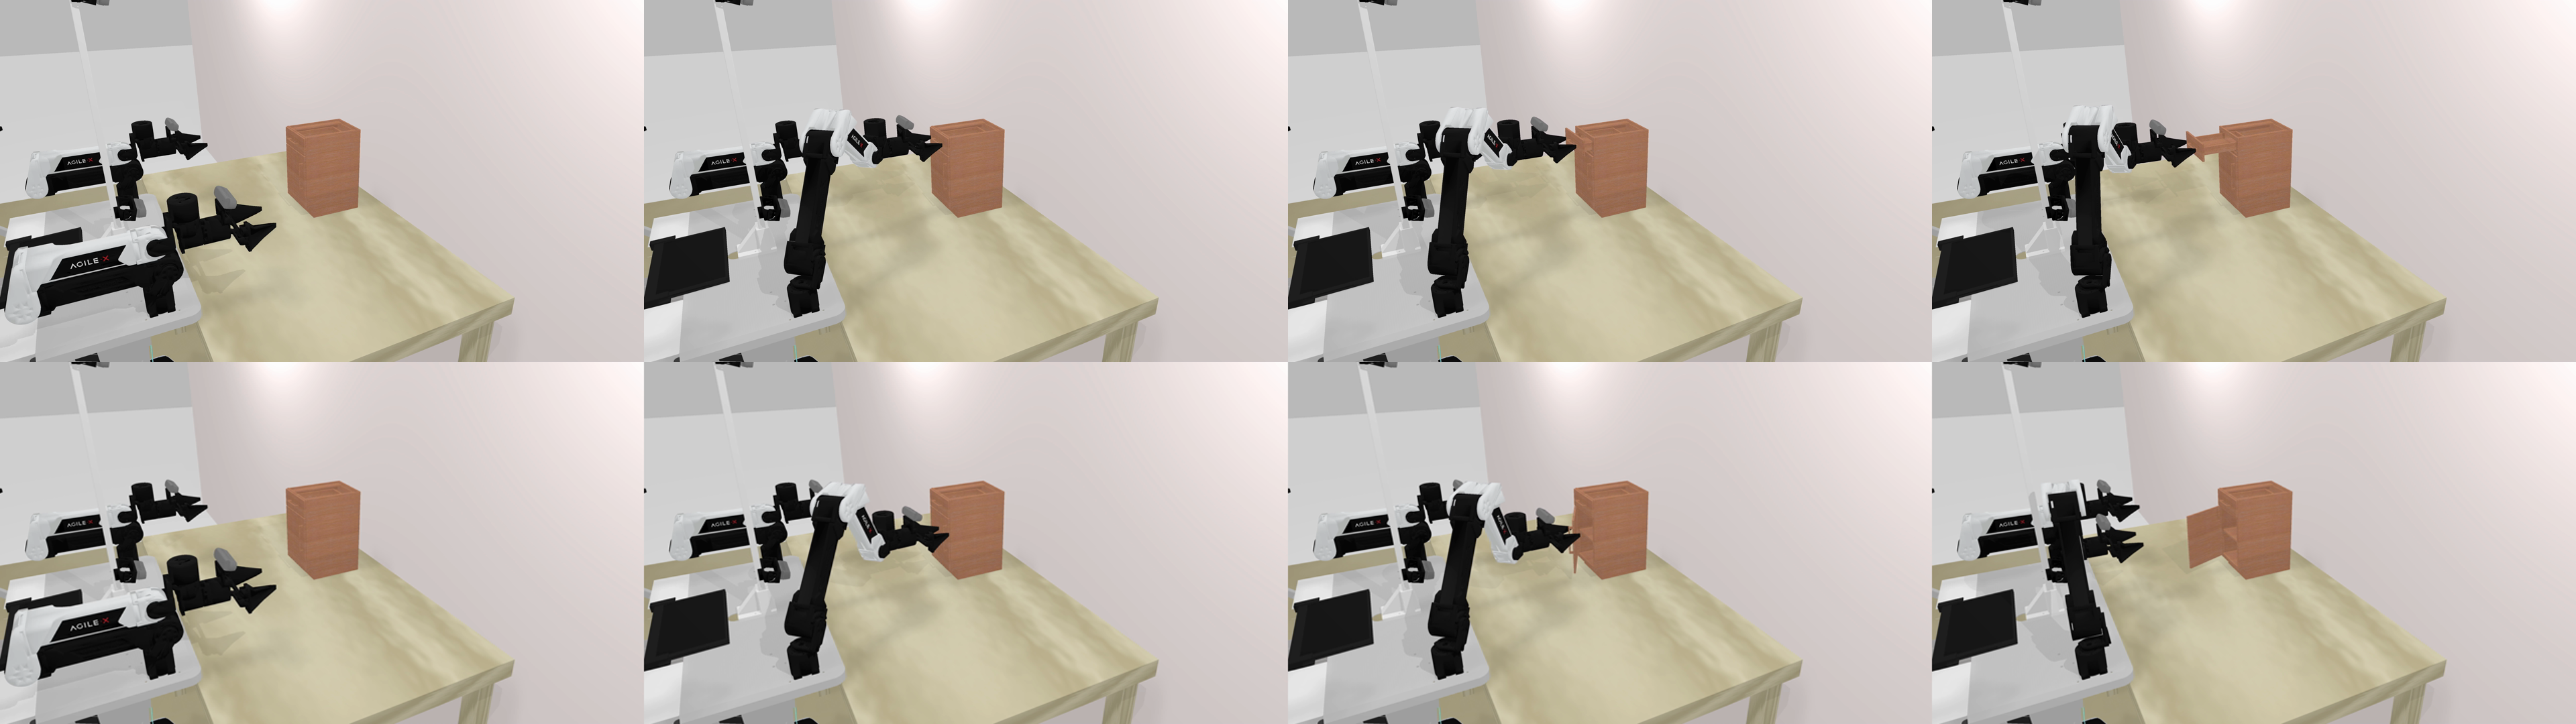
\includegraphics[width=\textwidth]{figs/4_application.png}
  \caption{\textbf{RoboTwin application with generated URDF assets.}
  We export \method{}'s predicted articulated structures as URDF assets and import them into RoboTwin.
  Each row shows four snapshots of contact-based manipulation: a drawer asset (top) and a door asset (bottom) are opened by a robot arm using the predicted movable link, joint axis, and motion range.}
  \label{fig:_application}
\end{figure}


\subsection{Application}
\label{sec:exp_application}

We further test whether the predicted articulation can be exported as a usable robot-simulation asset.
To this end, we convert the outputs to a URDF.
% predicted part masks into link meshes and instantiate the predicted kinematic tree, joint types, axes, and ranges as a URDF.
As shown in~\cref{fig:_application}, the generated drawer and door assets can be loaded into RoboTwin and opened by a robot arm through contact.
% This application checks a property that static reconstruction metrics do not directly measure.
For the robot to open the generated asset, the predicted movable part, joint axis, and motion range must remain mutually consistent under physics-based interaction.
The RoboTwin result, therefore, provides a compact qualitative validation that two-state geometry can support not only offline articulation recovery but also downstream manipulation of generated articulated assets.
